\documentclass[manuscript,screen,nonacm]{acmart}

\AtBeginDocument{%
  \providecommand\BibTeX{{Bib\TeX}}}

\setcopyright{none}
\settopmatter{printacmref=false}
\acmConference[]{}{}{}
\acmSubmissionID{}
\fancyfoot{}
\fancyfoot[C]{\thepage}

\usepackage{amsmath}
\usepackage{booktabs}
\usepackage{float}
\usepackage{graphicx}

\begin{document}

\title{Do Internal Trajectories Track Terminal Reward?\\
A Pilot Study Across OLMo 3 Checkpoints}

\author{Tenny Liu}
\email{zl6113@nyu.edu}
\affiliation{%
  \institution{Center for Data Science, New York University}
  \country{USA}
}
\renewcommand{\shortauthors}{Tenny Liu}

\maketitle

\section*{Executive Summary}

This pilot study asks whether intermediate language-model representations and
token-level confidence correspond to terminal instruction-following reward.
I evaluated matched OLMo 3 Base, SFT, DPO, and RLVR checkpoints on six
instruction-following prompts, with five stochastic rollouts per prompt and
checkpoint. This produced 120 responses. Each response was scored with an
IFEvalG constraint verifier, and hidden states and confidence statistics were
recorded at 25\%, 50\%, 75\%, and 100\% of generation.

Mean verifier reward increased modestly from 0.102 for Base to 0.137 for RLVR,
but the change was concentrated in one prompt rather than distributed across
the evaluation set. For SFT, DPO, and RLVR, confidence was positively
correlated with reward early in generation but weakly or negatively correlated
at completion. Activation movement exhibited checkpoint-specific correlations,
including a terminal Pearson correlation of 0.390 for DPO, but no consistent
pattern across checkpoints. The held-out reward probes were not evaluable:
both test prompts had reward zero for every rollout, making held-out $R^2$
undefined. In addition, every response reached the 128-token cap. The results
therefore establish a working measurement pipeline and reveal descriptive
confidence--behavior divergence, but they do not establish reliable reward
decodability, causal faithfulness, or model generalization.

\begin{figure}[H]
    \centering
    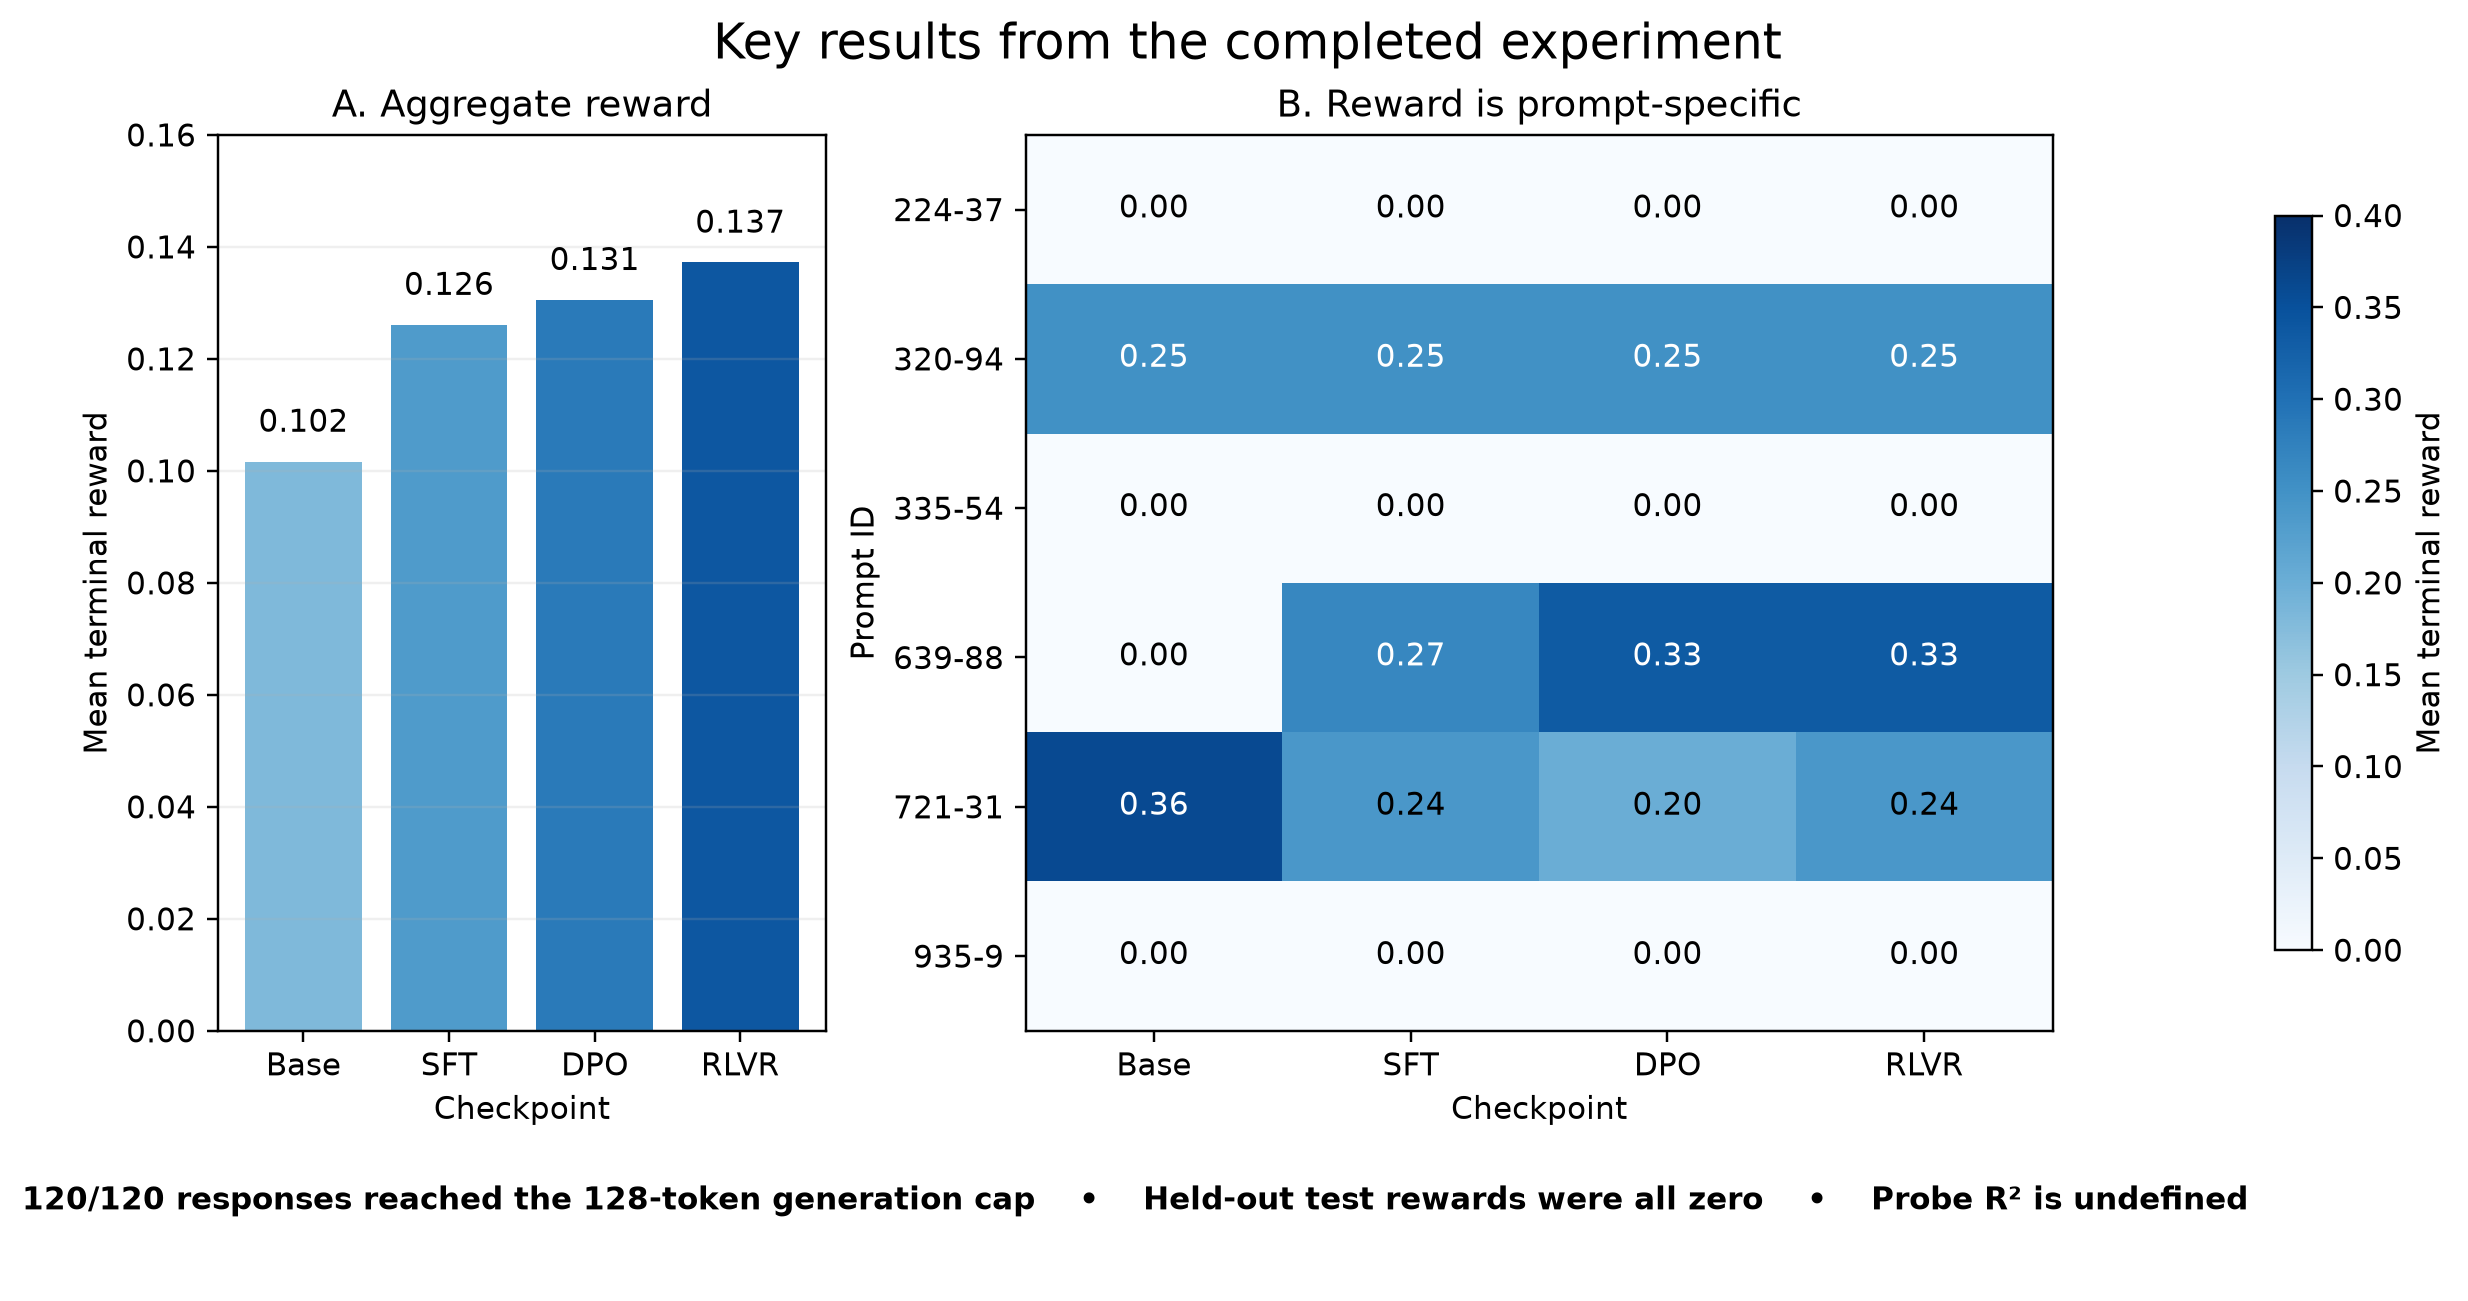
\includegraphics[width=0.94\linewidth]{figures/executive_summary.png}
    \caption{Key outcomes from the completed 120-rollout experiment. Aggregate
    reward changes were small, prompt effects were large, every response hit
    the generation cap, and the held-out reward target had zero variance.}
    \label{fig:executive-summary}
\end{figure}

\clearpage

\section{Introduction}

Reinforcement learning for language models commonly assigns reward after a
complete response has been generated. The terminal score indicates whether an
outcome met an external objective, but it does not reveal when information
about that outcome became available inside the model. If intermediate hidden
states contain outcome-relevant information, they may support monitoring of a
generation before the terminal verifier is applied. If inexpensive confidence
statistics contain the same information, they may provide a simpler signal.
Conversely, confidence may rise even when a response violates externally
specified constraints.

This work studies that distinction in a small, controlled instruction-following
setting. IFEval-style prompts are useful because they attach deterministic,
programmatically checkable constraints to natural-language responses
\citep{zhou2023ifeval}. I compare four publicly released checkpoints from the
same OLMo model family, reducing architectural differences relative to a
comparison of unrelated models \citep{groeneveld2024olmo,olmo3card}.

The study asks three questions:

\begin{enumerate}
    \item How do hidden-state movement and policy confidence evolve during a
    rollout, and how are they associated with terminal verifier reward?
    \item Which instruction constraints are passed or failed across the four
    checkpoints?
    \item Can a linear probe trained on intermediate state predict terminal
    reward on held-out prompt groups?
\end{enumerate}

These questions concern \emph{internal--behavioral correspondence}. A
correlation or successful probe would show that outcome information is
available in a representation; it would not show that the representation
causes the behavior. Similarly, the comparison across checkpoints is
descriptive. Although prior work has contrasted memorization under SFT with
generalization under outcome-based RL \citep{chu2025sft}, the present data do
not provide the unseen task variants required to test that claim.

\section{Methods}

\subsection{Experimental Design and Checkpoints}

The experiment used four OLMo 3 7B checkpoints:

\begin{itemize}
    \item \textbf{Base}: \texttt{allenai/Olmo-3-1025-7B};
    \item \textbf{SFT}: \texttt{allenai/Olmo-3-7B-Think-SFT};
    \item \textbf{DPO}: \texttt{allenai/Olmo-3-7B-Think-DPO}; and
    \item \textbf{RLVR}: \texttt{allenai/Olmo-3-7B-Think}.
\end{itemize}

For every checkpoint, the model generated five stochastic rollouts for each of
six prompts. Generation used temperature 0.6, top-$p$ 0.95, random seed 0,
and a maximum of 128 new tokens. The same prompt IDs and generation settings
were used for all checkpoints. The resulting dataset contains

\begin{equation}
4\ \text{checkpoints}\times 6\ \text{prompts}\times
5\ \text{rollouts}=120\ \text{responses}.
\end{equation}

\subsection{Prompt Source}

Prompts were streamed from revision
\texttt{0fb6466d31ef3a9dd16985ef635e6429e05a6491} of
\texttt{allenai/Dolci-Think-RL-7B}. The loader selected examples whose
\texttt{original\_dataset} field was
\texttt{hamishivi/IF\_multi\_constraints\_upto5\_filtered}. This source was
part of the data used for OLMo 3 RLVR training \citep{dolcirl}. Consequently,
the experiment measures behavior on an RLVR training-source distribution, not
on a held-out task distribution.

\subsection{Terminal Reward}

Each completed response was evaluated with the IFEvalG instruction registry
from Ai2's \texttt{open-instruct} implementation \citep{openinstruct}. If a
prompt specifies $m$ constraints, terminal reward is

\begin{equation}
R_T=\frac{1}{m}\sum_{j=1}^{m}
\mathbb{I}[\text{constraint}_j\ \text{is satisfied}].
\end{equation}

The analysis retained both $R_T$ and the binary result for every individual
constraint. Reward therefore measures the fraction of requested formatting or
lexical constraints satisfied; it is not a general measure of factual quality.

\subsection{Trajectory Measurements}

After generation, the prompt and completed response were passed through the
same checkpoint again with hidden-state output enabled. Measurements were
taken at the generated token nearest each trajectory fraction

\begin{equation}
t/T\in\{0.25,0.50,0.75,1.00\}.
\end{equation}

Residual-stream vectors were retained from transformer layers
$\ell\in\{8,16,24,32\}$. Each saved activation is a single-token vector, not a
mean-pooled response representation. For descriptive plots, final-layer
movement relative to the 25\% position was measured as

\begin{equation}
D_t=\frac{\lVert h^{(32)}_t-h^{(32)}_{0.25T}\rVert_2}{\sqrt{d}}.
\end{equation}

Thus $D_{0.25T}=0$ by construction. For predictive analysis, the implementation
also formed adjacent differences $\Delta h_t=h_t-h_{t-1}$.

For every generated token, the implementation computed chosen-token log
probability, predictive entropy, and top-1 next-token probability. Prefix means
and last-token values were saved at each trajectory fraction. Descriptive
confidence was the geometric mean sampled-token probability

\begin{equation}
C_t=\exp\left(\frac{1}{t}\sum_{i=1}^{t}
\log p_\theta(y_i\mid x,y_{<i})\right).
\end{equation}

This is a policy sharpness measure, not a calibrated probability that the
response will satisfy the verifier.

\subsection{Descriptive Analyses}

For each checkpoint and trajectory fraction, Pearson and Spearman correlations
were computed for $C_t$ versus $R_T$, $D_t$ versus $R_T$, and $C_t$ versus
$D_t$. Constraint pass rates were calculated separately by verifier instruction
ID and checkpoint. These statistics pool the 30 rollouts from each checkpoint;
because five rollouts share each prompt, they are treated as descriptive rather
than as independent inferential observations.

\subsection{Held-Out Reward Probes}

Ridge-regression probes were fit separately for each checkpoint, layer, and
trajectory fraction. The implemented feature sets were:

\begin{enumerate}
    \item current activation $h_t$;
    \item concatenated activation history $[h_{0.25T};\ldots;h_t]$;
    \item adjacent activation change $\Delta h_t$;
    \item six policy-confidence statistics; and
    \item current activation combined with confidence statistics.
\end{enumerate}

The Base checkpoint served as the model baseline. No TF--IDF baseline was used.
One fixed 75/25 split was grouped by prompt, placing four prompt groups in the
training set and two in the test set. All five rollouts from a prompt remained
in the same split. The statistical null permuted complete prompt-level blocks
of training rewards before refitting each probe. Recorded metrics included
held-out $R^2$, mean squared error, rank correlation, and the prompt-block
permutation distribution.

\section{Results}

\subsection{Terminal Reward Varied More by Prompt Than by Checkpoint}

Table~\ref{tab:reward-summary} reports aggregate verifier reward. Mean reward
rose from 0.1017 for Base to 0.1372 for RLVR, an absolute difference of 0.0355.
The increase was not broad across prompts. Three prompts received reward zero
for every checkpoint, and one prompt received exactly 0.25 for every
checkpoint. Prompt 639-88 improved from 0.0000 for Base to 0.3333 for DPO and
RLVR, whereas prompt 721-31 decreased from 0.3600 for Base to 0.2400 for RLVR.
Figure~\ref{fig:executive-summary} displays this heterogeneity.

\begin{table}[t]
\centering
\caption{Terminal verifier reward across 30 rollouts per checkpoint. Standard
deviations describe rollout-level variation and do not adjust for clustering by
prompt.}
\label{tab:reward-summary}
\begin{tabular}{lrrrr}
\toprule
Checkpoint & Mean & SD & Minimum & Maximum \\
\midrule
Base & 0.1017 & 0.1534 & 0.0000 & 0.4000 \\
SFT  & 0.1261 & 0.1438 & 0.0000 & 0.4000 \\
DPO  & 0.1306 & 0.1386 & 0.0000 & 0.3333 \\
RLVR & 0.1372 & 0.1466 & 0.0000 & 0.4000 \\
\bottomrule
\end{tabular}
\end{table}

All 120 generations contained exactly 128 generated tokens. The maximum-token
limit therefore censored every response, including responses evaluated with
completion-sensitive constraints.

\subsection{Constraint Outcomes Were Sparse and Highly Specific}

Figure~\ref{fig:constraint-pass-rates} shows the observed constraint pass
rates. The exclude-word and palindrome constraints were passed in every
rollout for every checkpoint. In contrast, JSON formatting, first-word,
same-start/end, required-last-word, paragraph-first-word, exact-word-count, and
counting-composition constraints were never passed in this sample.

\begin{figure}[t]
    \centering
    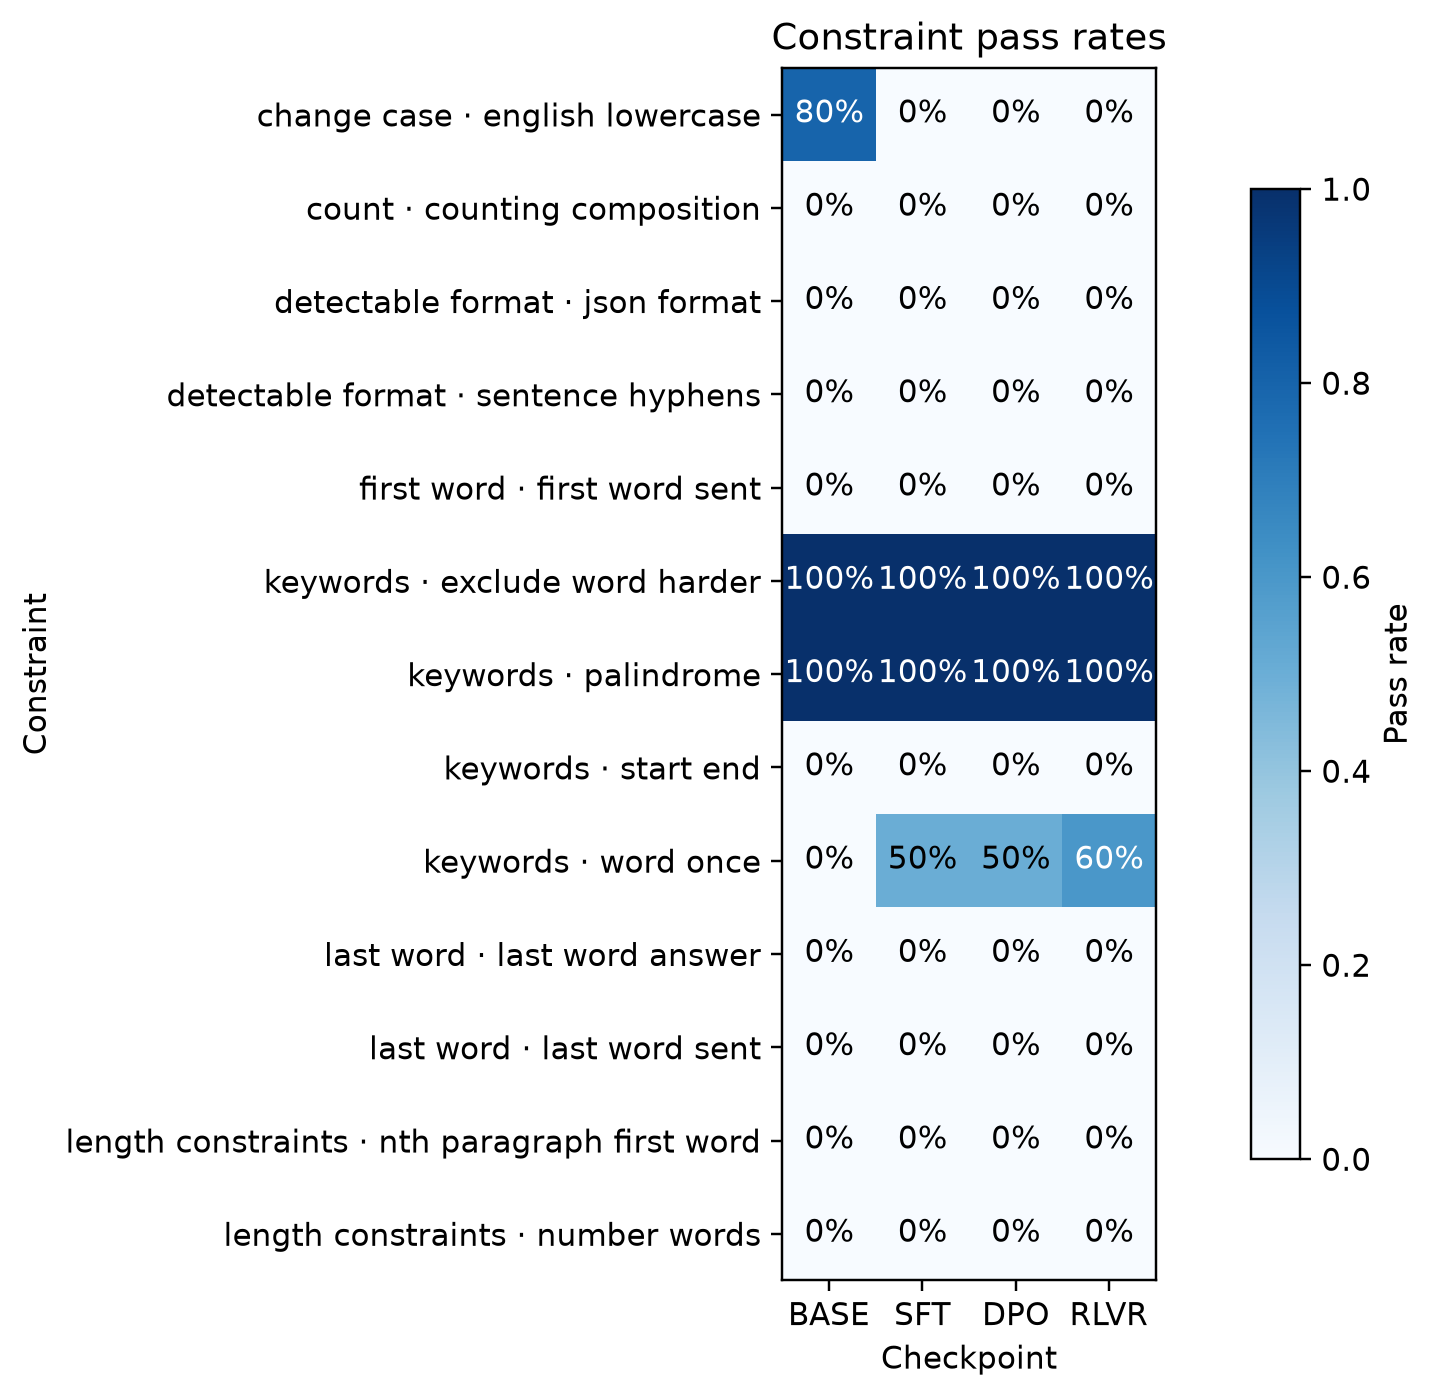
\includegraphics[width=0.90\linewidth]{figures/constraint_pass_rates.png}
    \caption{Observed pass rate for each verifier constraint and checkpoint.
    Each cell is the fraction of evaluated instances that passed. Counts are
    omitted because most constraint IDs occur in only one of the sampled
    prompts.}
    \label{fig:constraint-pass-rates}
\end{figure}

The clearest post-training increase occurred for the requirement that a
specified word appear exactly once: its pass rate was 0\% for Base, 50\% for
SFT, 50\% for DPO, and 60\% for RLVR. The lowercase requirement showed the
opposite pattern, with 80\% for Base and 0\% for all three post-trained
checkpoints. Because constraint identity is nearly confounded with prompt
identity in this sample, these values describe the six selected prompts rather
than general constraint-level capabilities.

\subsection{Confidence and Activation Movement Followed Different Trajectories}

Mean generated-token confidence increased across the Base trajectory, from
0.626 at 25\% to 0.698 at completion. In contrast, mean confidence decreased
over generation for SFT (0.821 to 0.736), DPO (0.890 to 0.853), and RLVR
(0.865 to 0.817). Post-trained checkpoints nevertheless remained more
confident on average than Base at every sampled fraction.

Final activation-change RMS was 1.473 for Base, 1.776 for SFT, 1.803 for DPO,
and 1.809 for RLVR. These values indicate larger movement away from the 25\%
state in the post-trained checkpoints, but movement magnitude alone does not
identify a reward-relevant direction.

Figure~\ref{fig:trajectory-correlations} shows Pearson correlations with
terminal reward. For SFT, DPO, and RLVR, confidence--reward correlation began
positive at 25\% (0.560, 0.586, and 0.557 respectively) and fell during the
rollout. At completion, the correlations were $-0.110$, $-0.261$, and
$-0.374$. Base remained weakly positive, ending at 0.210.

\begin{figure}[t]
    \centering
    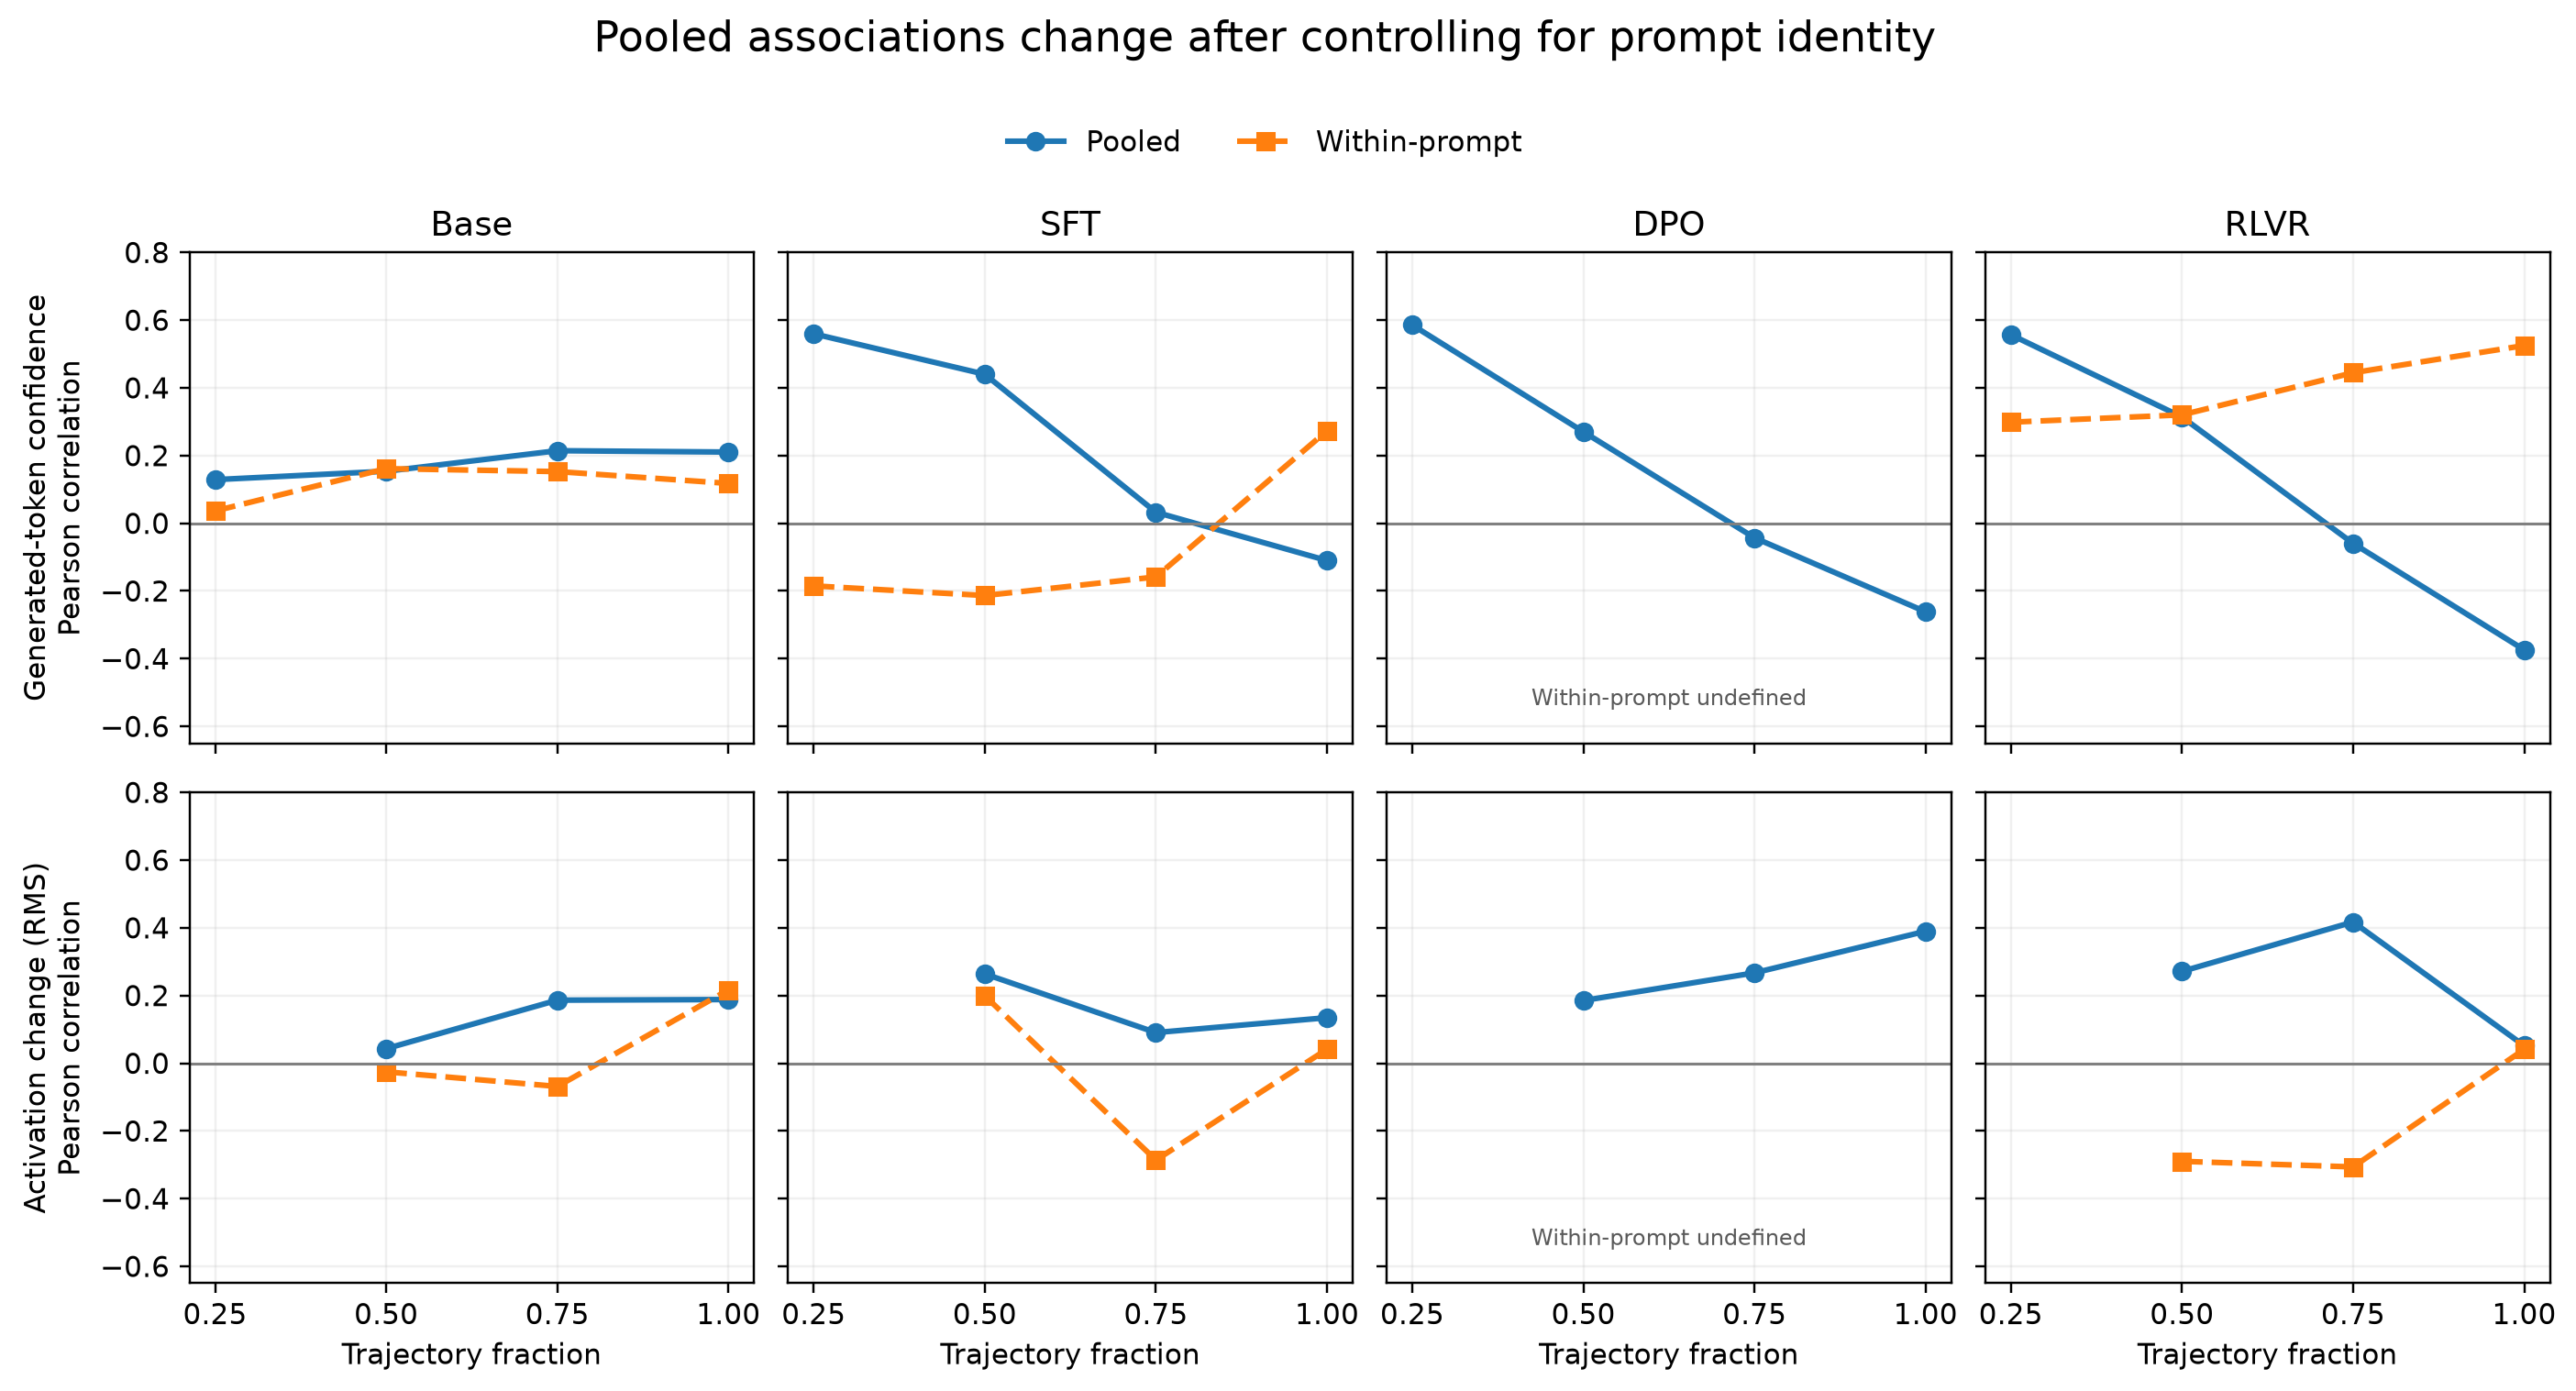
\includegraphics[width=\linewidth]{figures/trajectory_correlation_with_terminal_reward.png}
    \caption{Pearson correlation of generated-token confidence and final-layer
    activation-change RMS with terminal reward. Activation change at 25\% is
    undefined because that position is the zero-distance reference. Values are
    descriptive and pool rollouts within checkpoint.}
    \label{fig:trajectory-correlations}
\end{figure}

Activation-change correlation was not consistent across checkpoints. DPO rose
from 0.185 at 50\% to 0.390 at completion. RLVR rose from 0.271 at 50\% to
0.417 at 75\%, then fell to 0.052 at completion. SFT and Base ended at 0.134
and 0.188. These patterns show that policy confidence and representation
movement are not interchangeable measurements, but the sample does not support
an inferential claim that either reliably tracks reward.

\subsection{Held-Out Reward Decodability Was Not Evaluable}

The fixed split assigned prompts 335-54 and 935-9 to the test set. Both prompts
received terminal reward zero in all five rollouts from all four checkpoints.
Consequently, test-target variance was zero for every probe evaluation.
Held-out $R^2$ and rank correlation were therefore undefined across all 256
checkpoint, layer, fraction, and feature-set combinations.

Mean squared error can still be calculated against a constant target, but it
does not measure discrimination between successful and unsuccessful held-out
outcomes. The shuffled-label null likewise cannot repair the missing outcome
variation. Accordingly, this experiment yields no evidence for or against
linear terminal-reward decodability. It instead identifies a data-coverage
failure in the pilot evaluation.

\section{Discussion}

The most defensible finding is a divergence between token-level confidence and
verified instruction following. The post-trained checkpoints generated tokens
with higher average probability than Base, yet their confidence--reward
correlations became weak or negative near completion. In this sample, a sharp
next-token distribution was therefore not a reliable substitute for the
external constraint verifier. This matters for reward design: optimizing policy
confidence alone could reinforce fluent, high-probability continuations that
still miss exact output requirements.

The activation results are more tentative. Post-trained checkpoints moved
farther from their 25\% hidden state than Base, and DPO showed a moderate
positive terminal association between movement magnitude and reward. RLVR's
association peaked at 75\% and nearly disappeared by completion. Because RMS
distance discards direction, these results do not show that the state moved
toward a shared ``reward direction.'' The held-out probe was intended to test
directional, linearly accessible information, but constant test outcomes made
that analysis uninformative.

Behavioral changes were also prompt-specific. The aggregate Base-to-RLVR gain
was largely explained by prompt 639-88 and its exactly-once keyword constraint,
while several structural requirements remained unsatisfied. The fact that all
responses reached the token limit offers a plausible measurement explanation
for failures involving final words, complete JSON, and exact document
structure. It does not explain failures on every constraint, but it prevents a
clean capability interpretation.

Finally, the checkpoint comparison cannot distinguish memorization from
generalization. The prompts came from the RLVR training-source dataset, and the
four checkpoints represent sequential stages rather than independently
controlled SFT and RL treatments. The results can describe how these released
checkpoints behaved; they cannot establish that RL generalized a capability
already present in Base.

\section{Limitations}

\paragraph{Small number of prompt groups.}
The 120 responses contain only six distinct prompts. Repeated rollouts estimate
sampling variation for those prompts but do not substitute for broader prompt
coverage. Prompt identity is also strongly associated with both reward and
constraint identity.

\paragraph{Universal length censoring.}
Every response reached the 128-token maximum. The measured reward therefore
combines instruction-following performance with truncation effects.

\paragraph{Degenerate held-out target.}
Both test prompts had constant zero reward. The central held-out probe analysis
could not measure reward discrimination, and no conclusion about reward
decodability follows from this run.

\paragraph{Training-source evaluation.}
The sampled prompts came from the dataset used for RLVR training. The results do
not measure model generalization to unseen examples or task variants.

\paragraph{Checkpoint and trajectory confounding.}
Each checkpoint generated its own continuation. Cross-checkpoint activation
differences may therefore reflect both changed weights and changed tokens.

\paragraph{Coarse, single-token activation sampling.}
Only four positions and four layers were retained. Each activation represents
one token position rather than a pooled or token-complete trajectory, so brief
or distributed signals may be missed.

\paragraph{Observational analysis.}
Correlations and probes test association and decodability. No activation
intervention was performed, so the experiment does not establish causal
faithfulness.

\paragraph{Narrow external objective.}
IFEvalG reward measures explicit verifiable constraints. It does not measure
all aspects of factual correctness, usefulness, or human preference.

\section{Conclusion}

This study implemented an end-to-end pipeline connecting stochastic language
model rollouts, exact terminal constraint rewards, intermediate hidden states,
and policy-confidence statistics across Base, SFT, DPO, and RLVR checkpoints.
On the completed pilot, average reward increased slightly across post-training,
but performance was dominated by prompt-specific constraints. Confidence and
terminal reward diverged late in post-trained trajectories, while
activation-change associations varied by checkpoint and time. Because the
held-out test rewards were constant, the experiment did not establish terminal
reward decodability. The principal outcome is therefore a validated measurement
pipeline and a precise account of which data limitations prevent stronger
claims.

\section{Acknowledgments}

This work was prepared as application material for the MATS 12.0 Winter
2026--27 Neel Nanda Stream. AI assistants were used for implementation support,
debugging, figure generation, and manuscript editing. All numerical results in
the paper were recomputed from the saved rollout and activation artifacts.

\begin{thebibliography}{9}

\bibitem[Allen Institute for AI(2025a)]{olmo3card}
Allen Institute for AI.
\newblock OLMo 3 7B Think SFT model card.
\newblock \url{https://huggingface.co/allenai/Olmo-3-7B-Think-SFT}, 2025.

\bibitem[Allen Institute for AI(2025b)]{dolcirl}
Allen Institute for AI.
\newblock Dolci-Think-RL-7B dataset card.
\newblock \url{https://huggingface.co/datasets/allenai/Dolci-Think-RL-7B}, 2025.

\bibitem[Allen Institute for AI(2025c)]{openinstruct}
Allen Institute for AI.
\newblock Open Instruct.
\newblock \url{https://github.com/allenai/open-instruct}, 2025.

\bibitem[Chu et~al.(2025)]{chu2025sft}
Tianzhe Chu, Yuexiang Zhai, Jihan Yang, Shengbang Tong, Saining Xie,
Dale Schuurmans, Quoc~V. Le, Sergey Levine, and Yi Ma.
\newblock SFT memorizes, RL generalizes: A comparative study of foundation
model post-training.
\newblock \emph{arXiv preprint arXiv:2501.17161}, 2025.

\bibitem[Groeneveld et~al.(2024)]{groeneveld2024olmo}
Dirk Groeneveld et~al.
\newblock OLMo: Accelerating the science of language models.
\newblock \emph{Proceedings of ACL}, 2024.

\bibitem[Zhou et~al.(2023)]{zhou2023ifeval}
Jeffrey Zhou, Tianjian Lu, Swaroop Mishra, Siddhartha Brahma, Sujoy Basu,
Yi Luan, Denny Zhou, and Le Hou.
\newblock Instruction-following evaluation for large language models.
\newblock \emph{arXiv preprint arXiv:2311.07911}, 2023.

\end{thebibliography}

\appendix

\section{Implementation Summary}

The implementation contains the following components:

\begin{itemize}
    \item loading matched OLMo 3 Base, SFT, DPO, and RLVR checkpoints;
    \item streaming instruction-following prompts from a pinned revision of
    \texttt{Dolci-Think-RL-7B};
    \item sampling five stochastic rollouts per prompt and checkpoint;
    \item computing aggregate and individual IFEvalG constraint outcomes;
    \item extracting residual-stream states from four transformer layers at
    four trajectory fractions;
    \item computing prefix and last-token log probability, entropy, and top-1
    probability;
    \item fitting current-state, activation-history, activation-difference,
    confidence, and activation-plus-confidence Ridge probes;
    \item using a prompt-grouped fixed holdout and prompt-block shuffled-label
    null; and
    \item saving rollout, activation, prediction, correlation, plot, and W\&B
    artifact outputs.
\end{itemize}

The Base checkpoint is the model baseline. No TF--IDF history baseline or
POMDP simulation is part of the reported experiment.

\section{Example Prompt and Checkpoint Outcomes}

Prompt 639-88 asked the model to explain human digestion while satisfying three
verifiable constraints: paragraph 3 had to begin with \emph{art}, the keyword
\emph{being} had to appear exactly once, and the response had to end with
\emph{stroke}.

\begin{quote}
\small
``Can you list, explain, and give every individual reaction involved in the
process of human digestion from ingestion to excretion? There should be 4
paragraphs. Paragraphs and only paragraphs are separated with each other by two
new lines as if it was \texttt{'\textbackslash n\textbackslash n'} in python.
Paragraph 3 must start with word \emph{art}. Include keyword \emph{being} in
your response. The last word of your response should be the word
\emph{stroke}.''
\end{quote}

\begin{table}[H]
\centering
\small
\caption{Observed performance on prompt 639-88 across five rollouts per
checkpoint.}
\label{tab:example-prompt}
\begin{tabular}{l p{6.6cm} p{4.2cm} c}
\toprule
Checkpoint & Constraint outcomes & Per-rollout rewards & Mean \\
\midrule
Base & Passed none of the three constraints in all five rollouts. &
$[0,0,0,0,0]$ & 0.0000 \\
SFT & Passed the exactly-once keyword constraint in four of five rollouts;
failed both structural constraints in every rollout. &
$[0,\frac13,\frac13,\frac13,\frac13]$ & 0.2667 \\
DPO & Passed only the exactly-once keyword constraint in all five rollouts. &
$[\frac13,\frac13,\frac13,\frac13,\frac13]$ & 0.3333 \\
RLVR & Passed only the exactly-once keyword constraint in all five rollouts. &
$[\frac13,\frac13,\frac13,\frac13,\frac13]$ & 0.3333 \\
\bottomrule
\end{tabular}
\end{table}

\begin{figure}[H]
    \centering
    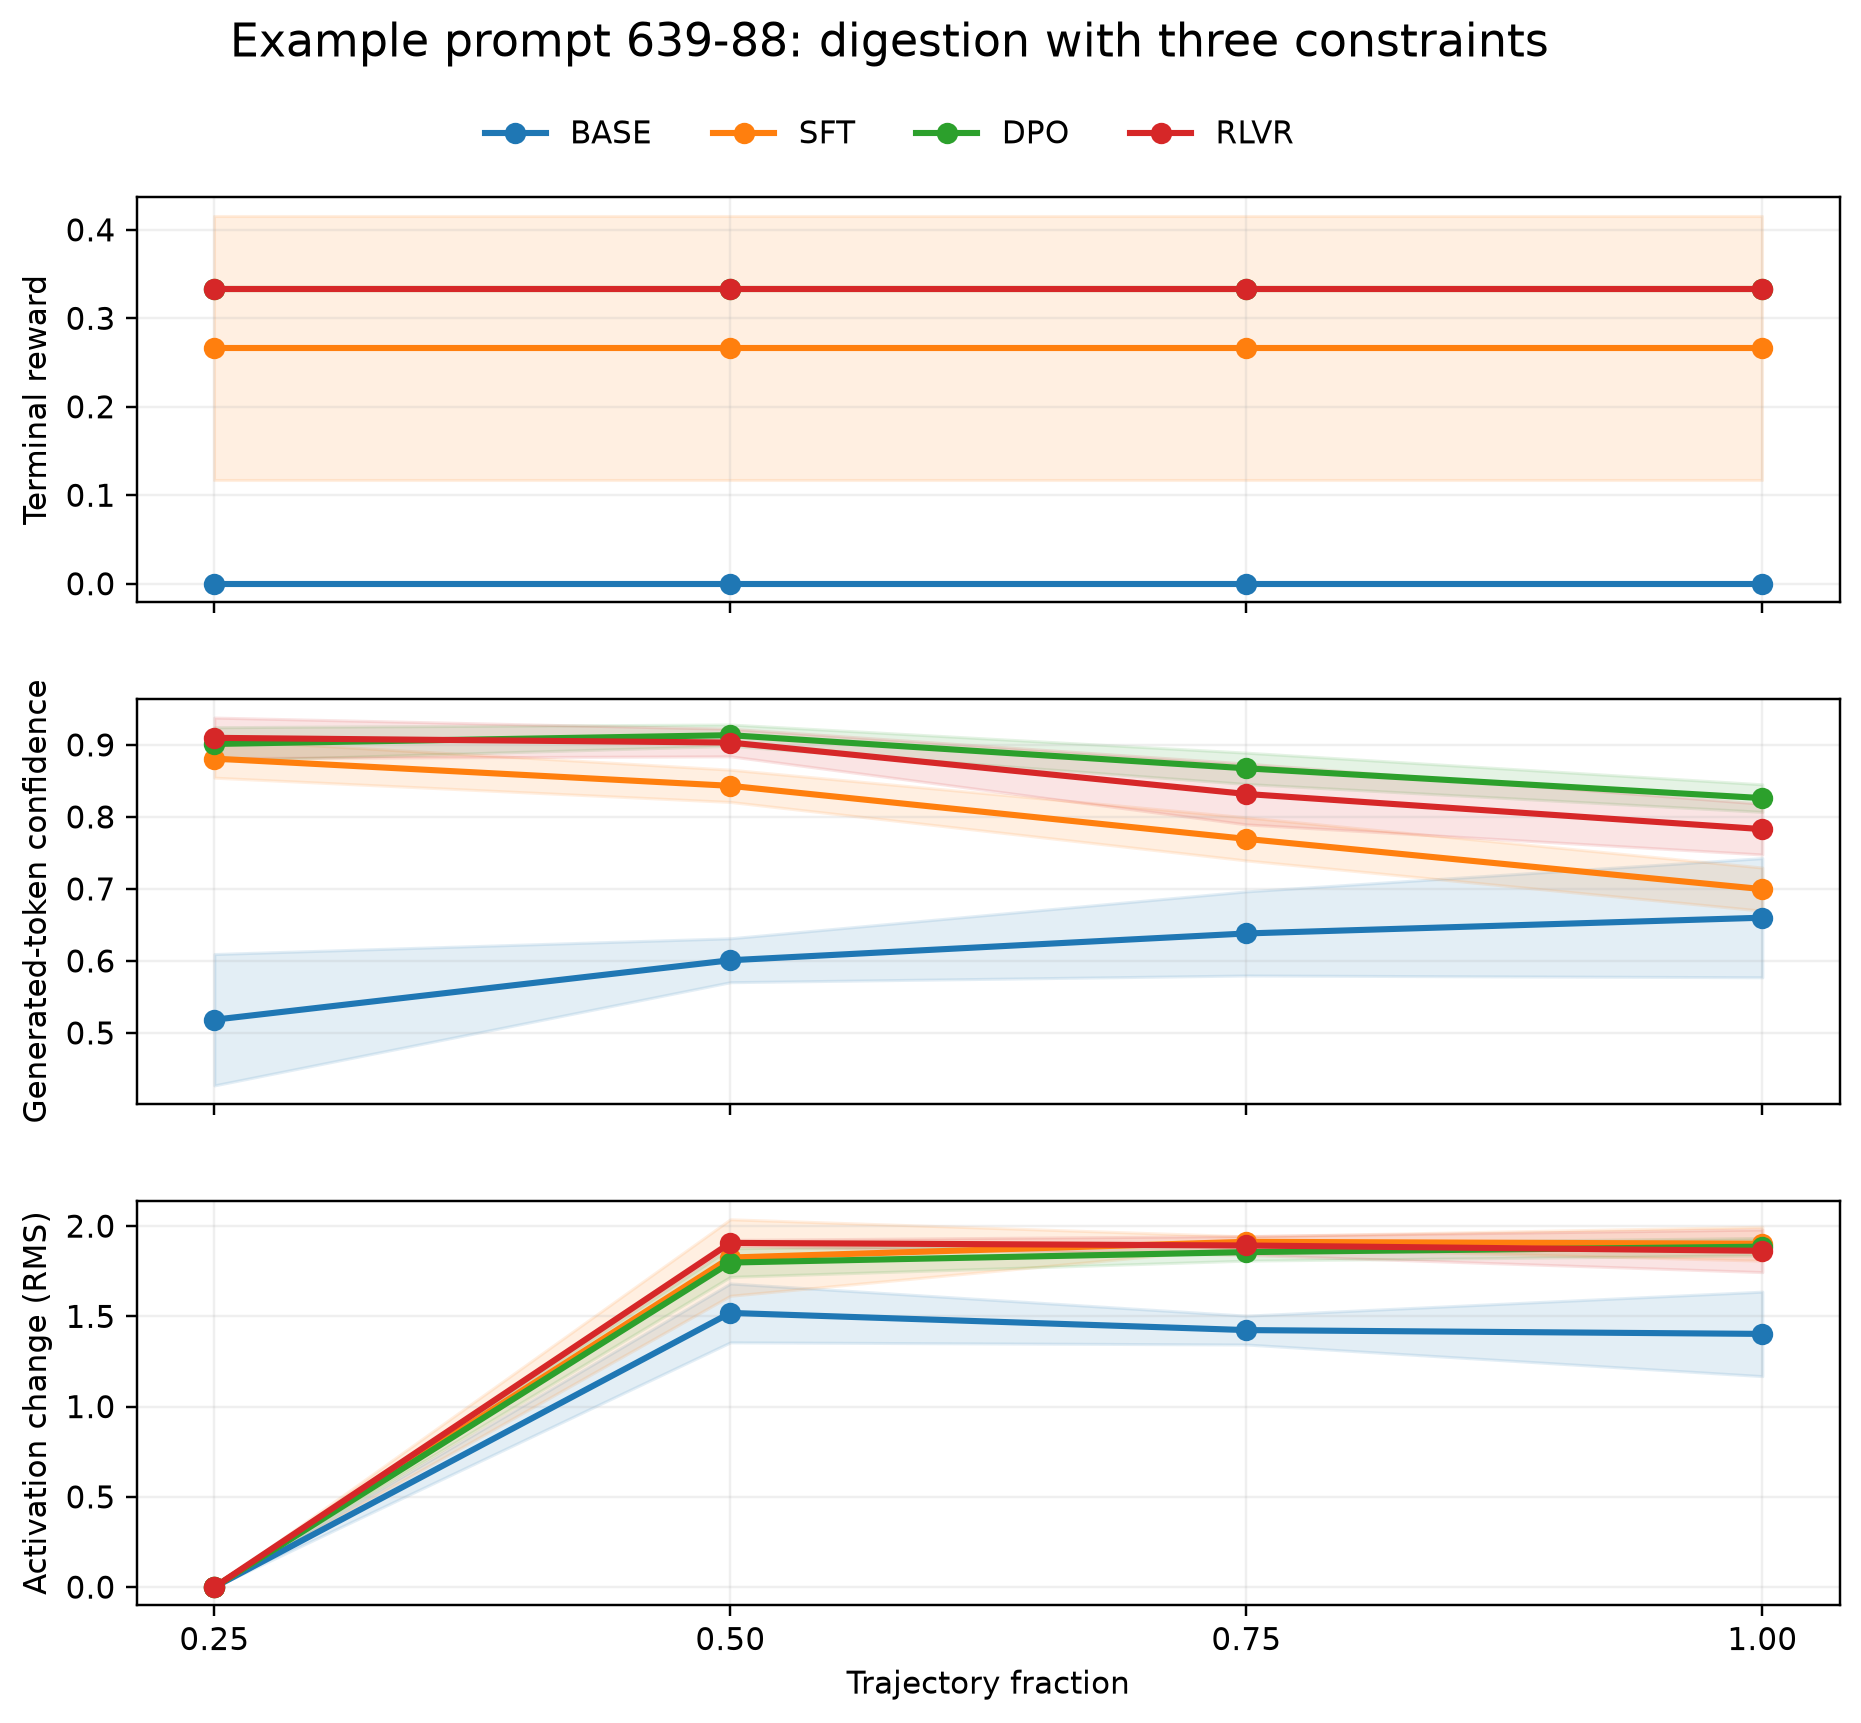
\includegraphics[width=\linewidth]{figures/example_prompt_639_88.png}
    \caption{Terminal reward, generated-token confidence, and final-layer
    activation-change RMS for prompt 639-88. Lines show means and shaded areas
    show standard deviations across five rollouts.}
    \label{fig:example-prompt}
\end{figure}

Post-training improved the lexical exactly-once requirement in this example,
but did not improve the paragraph-first-word or required-last-word constraints.
All responses reached the generation limit, which directly complicates the
interpretation of the required-last-word failure.

\section{Saved Analysis Artifacts}

The analysis produced \texttt{rollouts-annotated.jsonl},
\texttt{activations.npz}, \texttt{probe\_metrics.csv},
\texttt{heldout\_predictions.csv},
\texttt{instruction\_trajectories.csv},
\texttt{faithfulness\_correlations.csv},
\texttt{constraint\_difficulty.csv}, and
\texttt{constraint\_correlations.csv}. The code, figure generator, and paper
source are versioned in the accompanying repository.

\end{document}
